% !TeX program = xelatex
% Approved increment: textbook sections 1.9 through 1.12.
\documentclass[12pt,a4paper]{article}
\RequirePackage{array}[=2024-06-01]
% !TeX root = ../2/main.tex
\usepackage[a4paper,margin=25mm,headheight=16pt]{geometry}
\usepackage{amsmath,amssymb}
\usepackage{graphicx}
\usepackage{booktabs}
\usepackage{tabularx}
\usepackage{siunitx}
\usepackage{tikz}
\usepackage{circuitikz}
\usepackage[unicode,hidelinks]{hyperref}
\usepackage{xepersian}
% Only the regular B Nazanin file is installed; synthesize bold explicitly.
\settextfont[Path=C:/Windows/Fonts/,AutoFakeBold=2,AutoFakeSlant=0.2]{B-NAZANIN.TTF}
% B Nazanin lacks U+066A (Arabic percent), required by xepersian's digit setup.
% Arial covers the complete required digit/punctuation set; Persian prose remains B Nazanin.
\setdigitfont[Path=C:/Windows/Fonts/,BoldFont=arialbd.ttf,ItalicFont=ariali.ttf,BoldItalicFont=arialbi.ttf]{arial.ttf}
\setmathdigitfont[Path=C:/Windows/Fonts/,BoldFont=arialbd.ttf,ItalicFont=ariali.ttf,BoldItalicFont=arialbi.ttf]{arial.ttf}
\setlatintextfont{TeX Gyre Termes}
% B Nazanin does not contain the default itemize bullet and dash glyphs.
\renewcommand{\labelitemi}{\(\bullet\)}
\renewcommand{\labelitemii}{\(\circ\)}
\renewcommand{\labelitemiii}{\(\diamond\)}
\setlength{\parindent}{0pt}
\setlength{\parskip}{0.5em}
\linespread{1.25}
\newcommand{\exercise}[1]{\section*{تمرین #1}}
% !TeX root = ../2/main.tex
% Shared title page for every assignment.
% Change only \AssignmentNumber and \AssignmentDate in each main document.

\newcommand{\AssignmentNumber}[1]{\gdef\assignmentnumber{#1}}
\newcommand{\AssignmentDate}[1]{\gdef\assignmentdate{#1}}

\newcommand{\assignmentnumber}{---}
\newcommand{\assignmentdate}{---}

% Stable course metadata
\newcommand{\universityname}{دانشگاه صنعتی امیرکبیر}
\newcommand{\universityalias}{پلی‌تکنیک تهران}
\newcommand{\facultyname}{دانشکده مهندسی کامپیوتر}
\newcommand{\coursename}{طراحی مدارهای مجتمع پرتراکم پیشرفته}
\newcommand{\studentname}{محمد خلیلی اصل}
\newcommand{\instructorname}{دکتر مهدی صدیقی}

\newcommand{\MakeAssignmentCover}{%
  \begin{titlepage}
    \thispagestyle{empty}
    \centering
    \linespread{1}\selectfont

    \vspace*{0mm}
    
\includegraphics[width=44mm]{assets/aut-logo-black.png}\par
    \vspace{3mm}

    {\Large\bfseries \universityname\par}
    \vspace{1mm}
    {\large (\universityalias)\par}
    \vspace{1mm}
    {\large \facultyname\par}

    \vspace{8mm}
    {\Large\bfseries درس \coursename\par}

    \vspace{12mm}
    {\large عنوان\par}
    \vspace{2mm}
    {\LARGE\bfseries تمرین شماره \assignmentnumber\par}

    \vspace{10mm}
    {\large تهیه‌کننده\par}
    \vspace{2mm}
    {\Large\bfseries \studentname\par}

    \vspace{10mm}
    {\large استاد درس\par}
    \vspace{2mm}
    {\Large\bfseries \instructorname\par}

    \vspace{10mm}
    {\Large \assignmentdate\par}
    \vfill
  \end{titlepage}
  \setcounter{page}{1}%
}


\XeTeXgenerateactualtext=1
\newcommand{\secnum}[1]{\mbox{\beginL#1\endL}}
\newcommand{\code}[1]{\lr{\texttt{#1}}}
\setlength{\emergencystretch}{3em}
\widowpenalty=10000
\clubpenalty=10000
\AtBeginDocument{\DeclareSIPrefix{\micro}{\text{\lr{µ}}}{-6}}
\hypersetup{pdftitle={جزوه اول، از Circuit Design تا ساخت و آزمون}}
\AssignmentNumber{جزوه اول، از مدار تا تراشه}
\AssignmentDate{بخش‌های \secnum{۱.۹} تا \secnum{۱.۱۲} کتاب}
\patchcmd{\MakeAssignmentCover}{تمرین شماره \assignmentnumber}{\assignmentnumber}{}{\errmessage{Cover title replacement failed}}
\begin{document}
\MakeAssignmentCover
\section*{هدف و مسیر مطالعه}
در این بخش، توصیف منطقی به شبکه ترانزیستور، هندسه روی سیلیکون و در پایان
تراشه قابل‌آزمون تبدیل می‌شود. برای دنبال‌کردن متن، مفهوم ولتاژ، جریان، خازن،
گیت منطقی و جمع‌کننده کافی است. روابط لازم با تفسیر فیزیکی و محاسبه مرحله‌ای مرور می‌شوند.
هدف، درک وابستگی عملکرد، سرعت، توان و مساحت به انتخاب‌های طراحی است.

دامنه متن، بخش‌های \secnum{۱.۹} تا \secnum{۱.۱۲} کتاب، صفحات چاپی ۴۲ تا ۵۵ است
\cite{weste}. اسلاید ۱۷ مجموعه \lr{00} جایگاه این مراحل را در سطوح طراحی نشان می‌دهد
\cite{intro}. محاسبه‌های افزوده، شکل‌های شماتیک و تمرین‌های پاسخ‌دار جزوه آموزشی‌اند.
اعداد فناوری، چگالی، ابعاد و روش‌های ساخت برگرفته از کتاب با زمان و زمینه همان مرجع تفسیر می‌شوند.
هر جا داده فرضی به کار رود، فرض در متن معرفی می‌شود.

ابتدا تأخیر و توان و مثال \lr{Carry} را بررسی می‌کنیم. سپس \lr{Floorplan}،
\lr{Standard Cell}، \lr{Pitch Matching}، \lr{Slice Plan} و تخمین مساحت را می‌آموزیم.
در ادامه، روش‌های \lr{Verification} و مسیر \lr{Tapeout} تا \lr{Packaging} و \lr{Testing}
شرح داده می‌شوند. تمرین‌های پایانی هر بخش، پاسخ تشریحی دارند.
\tableofcontents
\clearpage
\section{طراحی در سطح مدار}
\label{sec:book-circuit-design}
\subsection{جریان و خازن چگونه تأخیر را تعیین می‌کنند؟}
در \lr{Circuit Design}، برای تابع منطقی مشخص، شبکه ترانزیستورها و اندازه آن‌ها
انتخاب می‌شود. خروجی یک گیت، ورودی گیت بعدی و سیم میان آن‌ها را راه‌اندازی می‌کند.
عایق \lr{Gate} موجب رفتار خازنی ورودی است. خازن‌های \lr{Diffusion} و سیم نیز به بار
خروجی افزوده می‌شوند. بنابراین صفر و یک‌شدن خروجی به جابه‌جایی بار الکتریکی نیاز دارد
\cite[بخش \secnum{۱.۹}، شکل \secnum{۱.۶۰}]{weste}.

اگر خازن معادل بار را \(C_L\) بنامیم، در مدل خازن ثابت رابطه بار و ولتاژ
\(Q=C_LV\) است. با تغییر ولتاژ به اندازه \(\Delta V\)، بار به اندازه
\(\Delta Q=C_L\Delta V\) تغییر می‌کند. جریان متوسط، بار جابه‌جاشده تقسیم بر زمان است.
از این دو تعریف، بدون نیاز به حل معادله دیفرانسیل، داریم
\begin{equation}
 I_{\mathrm{avg}}=\frac{\Delta Q}{\Delta t}
 \quad\Longrightarrow\quad
 \Delta t=\frac{C_L\Delta V}{I_{\mathrm{avg}}}.
 \label{eq:impl-charge-delay}
\end{equation}
برای جریان لحظه‌ای همین معنا به صورت \(i=C_L\,dV/dt\) نوشته می‌شود.
نماد \(dV/dt\) سرعت تغییر ولتاژ را بیان می‌کند. برای تخمین زمان تغییر کامل ولتاژ
از صفر تا \(V_{DD}\)، کتاب از تقریب
\begin{equation}
 t_{\mathrm{sw}}\approx\frac{C_LV_{DD}}{I_{\mathrm{avg}}}
 \label{eq:impl-full-swing}
\end{equation}
استفاده می‌کند. جریان ترانزیستور در طول گذار تغییر می‌کند، بنابراین انتخاب
\(I_{\mathrm{avg}}\) باید با همان بازه ولتاژ سازگار باشد. \lr{Propagation Delay}
معمولاً میان نقاط مرجع گذار ورودی و خروجی، مانند نصف ولتاژ تغذیه، اندازه‌گیری می‌شود.
رابطه \eqref{eq:impl-full-swing} یک تخمین مرتبه اول برای زمان تغییر ولتاژ است.

کنترل واحدها نتیجه را روشن می‌کند. چون \(\unit{\farad}=\unit{\coulomb\per\volt}\)
و \(\unit{\ampere}=\unit{\coulomb\per\second}\)، واحد
\(C_LV/I\) برابر ثانیه می‌شود. بار بیشتر، زمان بیشتر می‌خواهد. جریان قوی‌تر همان بار
را سریع‌تر جابه‌جا می‌کند. در مدل ایدئال، اگر \(C_L=0\) باشد این سهم از تأخیر صفر
می‌شود. اگر جریان به صفر نزدیک شود، زمان لازم افزایش می‌یابد.

در مثال فرضی، \(C_L=\qty{20}{\femto\farad}\)، \(V_{DD}=\qty{1}{\volt}\)
و \(I_{\mathrm{avg}}=\qty{100}{\micro\ampere}\) هستند. جای‌گذاری مرحله‌ای می‌دهد
\begin{equation*}
 t_{\mathrm{sw}}\approx
 \frac{20\times10^{-15}\times1}{100\times10^{-6}}\,\unit{\second}
 =2\times10^{-10}\,\unit{\second}=\qty{200}{\pico\second}.
\end{equation*}
دوبرابرشدن بار با جریان ثابت، زمان را به \qty{400}{\pico\second} می‌رساند.
این اعداد صرفاً برای تمرین تبدیل پیشوند و تحلیل رابطه انتخاب شده‌اند.

\subsection{اثر عرض ترانزیستور و بار مرحله بعد}
با ثابت‌بودن طول و شرایط بایاس، مدل مقدماتی جریان و خازن ورودی را متناسب با عرض
\(W\) می‌گیرد \cite[صفحه ۴۲]{weste}. افزایش عرض، جریان راه‌انداز و هم‌زمان بار
دیده‌شده در مرحله قبل را افزایش می‌دهد. اگر ضریب بزرگ‌کردن ترانزیستور \(s>0\)
باشد، برای تحلیل ساده می‌توان نوشت
\begin{equation}
 I(s)\approx sI_0,\qquad
 C_L(s)\approx C_{\mathrm{ext}}+sC_{\mathrm{int},0},\qquad
 t(s)\approx\frac{V_{DD}}{I_0}
 \left(\frac{C_{\mathrm{ext}}}{s}+C_{\mathrm{int},0}\right).
 \label{eq:impl-sizing}
\end{equation}
در این مدل، \(C_{\mathrm{ext}}\) بار ثابت خارجی و \(C_{\mathrm{int},0}\) سهم داخلی
در اندازه اولیه است. بزرگ‌کردن گیت، سهم بار ثابت را سریع‌تر راه‌اندازی می‌کند، اما
سهم خازن داخلی نیز رشد می‌کند. خازن ورودی بزرگ‌تر، تأخیر و انرژی مرحله قبل را تغییر
می‌دهد. انتخاب اندازه به مسیر چندمرحله‌ای، \lr{Fan-in}، \lr{Fan-out}، سیم و محدودیت
مساحت وابسته است. مدل‌های دقیق‌تر جریان و خازن در فصل ۲ و روش‌های اندازه‌گذاری در فصل ۴ آمده‌اند.

\subsection{استخراج انرژی و توان از شارژ خازن}
توان لحظه‌ای منبع تغذیه برابر \(p=V_{DD}i\) است. برای شارژ کامل یک خازن از صفر
تا \(V_{DD}\)، منبع بار \(Q=C_LV_{DD}\) تحویل می‌دهد. چون ولتاژ منبع ثابت است،
انرژی دریافت‌شده از منبع برابر می‌شود با
\begin{equation}
 E_{\mathrm{supply}}=V_{DD}Q=C_LV_{DD}^2.
 \label{eq:impl-supply-energy}
\end{equation}
انرژی ذخیره‌شده در خود خازن از جمع انرژی‌های کوچک \(V\,dQ\) به دست می‌آید.
با \(dQ=C_L\,dV\)، مساحت زیر خط \(C_LV\) از صفر تا \(V_{DD}\) یک مثلث است، پس
\begin{equation}
 E_C=\int_0^{V_{DD}}C_LV\,dV=\frac12 C_LV_{DD}^2.
 \label{eq:impl-stored-energy}
\end{equation}
در شارژ معمول مقاومتی، نیم دیگر انرژی منبع در مسیر شارژ تلف می‌شود. هنگام تخلیه،
انرژی ذخیره‌شده نیز در مسیر تخلیه تلف می‌شود. بنابراین انرژی یک چرخه کامل
\(0\rightarrow1\rightarrow0\) در این مدل برابر \(C_LV_{DD}^2\) است.

اگر در هر ثانیه \(f_{\mathrm{cyc}}\) چرخه کامل رخ دهد، توان متوسط برابر انرژی
هر چرخه ضرب‌در تعداد چرخه در ثانیه خواهد بود
\begin{equation}
 P_{\mathrm{dyn}}=C_LV_{DD}^2f_{\mathrm{cyc}}.
 \label{eq:impl-dynamic-power}
\end{equation}
این همان صورت رابطه کتاب است \cite[صفحه ۴۳]{weste}. برای ارتباط با \lr{Clock}،
\(\alpha_{01}\) را متوسط تعداد گذارهای \(0\rightarrow1\) در هر دوره \lr{Clock}
تعریف می‌کنیم. در حالت پایدار، فرکانس شارژ \(\alpha_{01}f_{\mathrm{clk}}\) است، پس
\begin{equation}
 P_{\mathrm{dyn}}=\alpha_{01}C_LV_{DD}^2f_{\mathrm{clk}}.
 \label{eq:impl-activity-power}
\end{equation}
با شمارش مجموع گذارهای صعودی و نزولی، باید تعریف ضریب فعالیت را نیز عوض کرد.
برای سیگنال متناوب \(0,1,0,1,\ldots\) در نمونه‌های متوالی \lr{Clock}، در هر دو
دوره یک شارژ رخ می‌دهد، بنابراین \(\alpha_{01}=1/2\) است. برای چند گره، سهم
\(\alpha_{01,k}C_kV_{DD}^2f_{\mathrm{clk}}\) هر گره جمع می‌شود.

در مثال فرضی \(C_L=\qty{20}{\femto\farad}\)، \(V_{DD}=\qty{1}{\volt}\)،
\(f_{\mathrm{clk}}=\qty{100}{\mega\hertz}\) و \(\alpha_{01}=0.25\)، داریم
\begin{equation}
 P_{\mathrm{dyn}}=0.25(20\times10^{-15})(1)^2(100\times10^6)
 \,\unit{\watt}=\qty{0.50}{\micro\watt}.
 \label{eq:impl-power-example}
\end{equation}
کاهش ولتاژ به \qty{0.8}{\volt} با ثابت‌فرض‌کردن سایر عوامل، توان را در
\(0.8^2=0.64\) ضرب می‌کند و به \qty{0.32}{\micro\watt} می‌رساند. جریان ترانزیستور
نیز به ولتاژ وابسته است، پس بررسی سرعت به مدل جریان نیاز دارد.

\subsection{توان \lr{Static} و انتخاب پیاده‌سازی}
ترانزیستور خاموش واقعی جریان نشتی دارد. اگر جریان متوسط مستقیم از تغذیه به زمین
را \(I_{\mathrm{static}}\) بنامیم، از تعریف توان به دست می‌آید
\begin{equation}
 P_{\mathrm{static}}=V_{DD}I_{\mathrm{static}}.
 \label{eq:impl-static-power}
\end{equation}
این رابطه حتی در نبود تغییر منطقی خروجی کاربرد دارد \cite[صفحه ۴۳]{weste}.
برای جریان فرضی \qty{10}{\nano\ampere} و تغذیه \qty{1}{\volt}، توان
\qty{10}{\nano\watt} است. مجموع این سهم و مثال \eqref{eq:impl-power-example}،
در مدل دو مؤلفه‌ای، \qty{0.51}{\micro\watt} می‌شود. جریان گذرای هم‌پوشانی روشن‌شدن
شبکه‌های \lr{Pull-up} و \lr{Pull-down} نیز می‌تواند سهم دیگری ایجاد کند که در تحلیل
تفصیلی فصل توان بررسی می‌شود.

\lr{Synthesis} با انتخاب گیت‌های کتابخانه و اندازه آن‌ها، تابع منطقی را تحت
محدودیت‌های طراحی پیاده می‌کند. \lr{Custom Circuit Design} امکان انتخاب شبکه
ترانزیستوری متناسب با تابع را فراهم می‌سازد. کتاب اهمیت آن را برای بخش‌های دارای
نیاز سرعت یا توان ویژه و برای حجم تولید توجیه‌کننده هزینه مهندسی توضیح می‌دهد.
\lr{Area}، توان، سرعت و تلاش طراحی باید هم‌زمان سنجیده شوند.

\subsection{مثال \lr{Carry} با ۲۶ و ۱۲ ترانزیستور}
در \lr{Full Adder}، ورودی‌های تک‌بیتی \(a,b,c\) هستند و \(c\) نقش \lr{Carry-in}
را دارد. خروجی \(c_{\mathrm{out}}\) وقتی یک می‌شود که دست‌کم دو ورودی یک باشند.
تابع آن برابر است با
\begin{equation}
 c_{\mathrm{out}}=ab+ac+bc.
 \label{eq:impl-carry-majority}
\end{equation}
در این معادله، کنارهم‌نوشتن نمادها به معنای \lr{AND} و علامت جمع به معنای
\lr{OR} است. برای مثال \(a=b=1\) با هر مقدار \(c\)، خروجی یک می‌دهد.
اگر فقط یک ورودی یک باشد، هر سه حاصل‌ضرب صفر می‌شوند.

پیاده‌سازی شکل \secnum{۱.۶۱} کتاب از سه \lr{AND2} و یک \lr{OR3} تشکیل می‌شود
\cite{weste}. \lr{AND2} در \lr{Static CMOS} معمول، یک \lr{NAND2} چهارترانزیستوری
و یک \lr{Inverter} دوترانزیستوری دارد. \lr{OR3} نیز از \lr{NOR3} شش‌ترانزیستوری
و یک \lr{Inverter} ساخته می‌شود. بنابراین
\begin{equation*}
 N_{\mathrm{gate}}=3(4+2)+(6+2)=26.
\end{equation*}
مسیر ورودی تا خروجی از چهار مرحله وارون‌کننده منطقی عبور می‌کند.
تأخیر هر مرحله تابع اندازه و بار آن است.

برای ساخت مدار فشرده، ابتدا تابع را عامل‌گیری می‌کنیم
\begin{equation}
 F=ab+c(a+b),\qquad c_n=\overline F,\qquad c_{\mathrm{out}}=\overline{c_n}.
 \label{eq:impl-factored-carry}
\end{equation}
شبکه \lr{Pull-down} گره \(c_n\)، یک شاخه دوترانزیستوری سری با کنترل \(a,b\)
و یک شاخه شامل \(c\) در سری با دو ترانزیستور موازی \(a,b\) دارد. این شبکه پنج
\lr{nMOS} می‌خواهد. هرگاه \(F=1\) باشد، مسیری تا زمین برقرار می‌شود.

شبکه \lr{Pull-up} شکل کتاب نیز پنج \lr{pMOS} دارد. شرط هدایت آن را با
\(\bar a,\bar b,\bar c\) بیان می‌کنیم، زیرا \lr{pMOS} با ورودی صفر روشن می‌شود.
با قانون \lr{De Morgan} و توزیع حاصل‌ضرب داریم
\begin{align*}
 \overline F
 &=(\bar a+\bar b)(\bar c+\bar a\bar b)\\
 &=\bar c(\bar a+\bar b)+\bar a\bar b.
\end{align*}
جمله اول، \(c\) در سری با موازی \(a,b\)، و جمله دوم، سری \(a,b\) در شبکه
\lr{pMOS} را مشخص می‌کند. بنابراین برای هر ورودی دودویی پایدار، یکی از شبکه‌ها
گره \(c_n\) را به تغذیه مناسب می‌رساند. \lr{Inverter} پایانی دو ترانزیستور دیگر دارد
و تعداد کل \(5+5+2=12\) می‌شود. مسیر منطقی شامل یک گیت مرکب و یک
\lr{Inverter} است. مقایسه سرعت عددی، به اندازه ترانزیستورها و بارها نیاز دارد.

جدول \ref{tab:impl-carry} همه حالت‌های دودویی را کنترل می‌کند. ستون \lr{PDN}
و \lr{PUN}، وجود مسیر رسانا برای گره \(c_n\) را نشان می‌دهند.
\begin{table}[ht]
\centering
\caption{کنترل کامل تابع و شبکه‌های \lr{Carry} در مدل سوئیچی ایدئال.}
\label{tab:impl-carry}
\begin{tabular}{ccccccc}
\toprule
\(a\)&\(b\)&\(c\)&\lr{PDN}&\lr{PUN}&\(c_n\)&\(c_{\mathrm{out}}\)\\
\midrule
۰&۰&۰&۰&۱&۱&۰\\
۰&۰&۱&۰&۱&۱&۰\\
۰&۱&۰&۰&۱&۱&۰\\
۰&۱&۱&۱&۰&۰&۱\\
۱&۰&۰&۰&۱&۱&۰\\
۱&۰&۱&۱&۰&۰&۱\\
۱&۱&۰&۱&۰&۰&۱\\
۱&۱&۱&۱&۰&۰&۱\\
\bottomrule
\end{tabular}
\end{table}

\subsection{\lr{Schematic} و دو سطح \lr{Netlist}}
\lr{Schematic} اتصال‌ها را به صورت تصویر و \lr{Netlist} همان ارتباط‌ها را به صورت
متن نمایش می‌دهد. در توصیف ساختاری گیت‌ها، نمونه آموزشی تابع \lr{Carry} چنین است
\cite[صفحات ۴۳ و ۴۴]{weste}.
\begin{latin}
\small
\begin{verbatim}
module carry(input logic a, b, c, output logic cout);
  logic x, y, z;
  and g1(x, a, b);
  and g2(y, a, c);
  and g3(z, b, c);
  or  g4(cout, x, y, z);
endmodule
\end{verbatim}
\end{latin}
در این \lr{Verilog}، نخستین آرگومان هر گیت خروجی است. نام‌های \code{g1} تا
\code{g4} شناسه نمونه‌ها و \code{x}، \code{y} و \code{z} سیم‌های میانی هستند.
گیت عمومی هنوز اندازه، خازن و مدل فناوری را مشخص نمی‌کند.

در توصیف سوئیچی کتاب، \code{tranif1} با کنترل یک و \code{tranif0} با کنترل صفر
اتصال برقرار می‌کنند. ترتیب آرگومان آن‌ها دو پایانه مسیر و سپس کنترل است.
برای نمونه \code{tranif1 n3(cn, i1, c)} گره‌های \code{cn} و \code{i1} را هنگام
یک‌بودن \code{c} وصل می‌کند. مسیر در این مدل دوطرفه است. \code{supply0} و
\code{supply1} به‌ترتیب زمین و تغذیه منطقی، و \code{tri} گره سیمی با قابلیت حالت
پرامپدانس را معرفی می‌کنند. این نمایش برای بررسی اتصال و عملکرد سوئیچی مناسب است.

برای تحلیل پیوسته ولتاژ، جریان، تأخیر و توان، \lr{SPICE} به مدل افزاره و ابعاد نیاز
دارد. ترانزیستور \lr{MOS} چهار پایانه \lr{Drain}، \lr{Gate}، \lr{Source} و
\lr{Body} دارد. خط معرفی آن در کتاب به ترتیب زیر است
\cite[صفحات ۴۴ و ۴۵]{weste}.
\begin{latin}
\small
\begin{verbatim}
Mname drain gate source body model W=width L=length
+ AD=drain_area AS=source_area
Cname node1 node2 value
\end{verbatim}
\end{latin}
علامت \code{+} در آغاز خط، ادامه همان دستور را نشان می‌دهد. \code{W} و
\code{L} عرض و طول کانال، و \code{AD} و \code{AS} مساحت‌های اتصال
\lr{Drain} و \lr{Source} هستند. نام مدل، پارامترهای فناوری را به نمونه مرتبط می‌کند.
این ترتیب با ترتیب آرگومان گیت‌های \lr{Verilog} تفاوت دارد.

فهرست \lr{SPICE} آموزشی زیر اتصال و ابعاد مثال کتاب را حفظ می‌کند. پسوندهای
\code{u}، \code{p} و \code{f} به‌ترتیب ضرایب \(10^{-6}\)، \(10^{-12}\) و
\(10^{-15}\) هستند. بنابراین \code{W=2u} طول \qty{2}{\micro\metre} و
\code{AD=1.8p} مساحت \qty{1.8}{\micro\metre\squared} را مشخص می‌کنند.
نام‌های گره و ترتیب درگاه‌ها از مرجع حفظ شده‌اند.
\begin{latin}
\footnotesize
\begin{verbatim}
.SUBCKT CARRY A B C COUT VDD GND
MN1 I1 A GND GND NMOS W=2u L=0.6u AD=1.8p AS=3p
MN2 I1 B GND GND NMOS W=2u L=0.6u AD=1.8p AS=3p
MN3 CN C I1 GND NMOS W=2u L=0.6u AD=3p AS=3p
MN4 I2 B GND GND NMOS W=2u L=0.6u AD=0.9p AS=3p
MN5 CN A I2 GND NMOS W=2u L=0.6u AD=3p AS=0.9p
MP1 I3 A VDD VDD PMOS W=4u L=0.6u AD=3.6p AS=6p
MP2 I3 B VDD VDD PMOS W=4u L=0.6u AD=3.6p AS=6p
MP3 CN C I3 VDD PMOS W=4u L=0.6u AD=6p AS=6p
MP4 I4 B VDD VDD PMOS W=4u L=0.6u AD=1.8p AS=6p
MP5 CN A I4 VDD PMOS W=4u L=0.6u AD=6p AS=1.8p
MN6 COUT CN GND GND NMOS W=4u L=0.6u AD=6p AS=6p
MP6 COUT CN VDD VDD PMOS W=8u L=0.6u AD=12p AS=12p
CI1 I1 GND 6f
CI3 I3 GND 9f
CA A GND 12f
CB B GND 12f
CC C GND 6f
CCN CN GND 12f
CCOUT COUT GND 6f
.ENDS CARRY
\end{verbatim}
\end{latin}
در نمونه \code{MN3}، \lr{Body} به زمین متصل است، هرچند \lr{Source} روی گره
داخلی \code{I1} قرار دارد. \lr{Body}های \lr{pMOS} به \code{VDD} وصل شده‌اند.
مدل ترانزیستور، سهم خازن‌های ذاتی و پیوندی را با استفاده از ابعاد محاسبه می‌کند.
خازن‌های صریح این مثال، سهم اضافی سیم‌کشی را نمایش می‌دهند. در شبکه‌های دارای
سیم بلند، مقاومت سیم نیز باید در مدل مناسب منظور شود.

این قطعه، تعریف \lr{Subcircuit} است. اجرای تحلیل به تعریف معتبر مدل‌های
\code{NMOS} و \code{PMOS}، منبع تغذیه، تحریک ورودی، بار و دستور تحلیل نیاز دارد.
پارامترهای مدل فناوری باید از منبع فناوری انتخاب‌شده تأمین شوند.

\subsection{تمرین‌های پاسخ‌دار \lr{Circuit Design}}
\textbf{تمرین ۱.} بار \qty{30}{\femto\farad} با تغییر ولتاژ \qty{0.8}{\volt}
در \qty{120}{\pico\second} شارژ می‌شود. جریان متوسط لازم چقدر است؟
از \eqref{eq:impl-charge-delay} با حل برای جریان داریم
\[
 I_{\mathrm{avg}}=\frac{30\times10^{-15}\times0.8}{120\times10^{-12}}
 \,\unit{\ampere}=\qty{200}{\micro\ampere}.
\]
توان \(10^{-15}/10^{-12}=10^{-3}\) و ضریب \(24/120=0.2\) است، بنابراین
\(0.2\times10^{-3}\,\unit{\ampere}=\qty{200}{\micro\ampere}\) می‌شود.

\textbf{تمرین ۲.} اگر خازن دو برابر، فرکانس نصف و ولتاژ ۱۰ درصد کمتر شود، با
ضریب فعالیت ثابت، نسبت توان جدید به قبلی چقدر است؟ با تقسیم دو بار
\eqref{eq:impl-activity-power} بر یکدیگر داریم
\[
 \frac{P_2}{P_1}=\frac{C_2}{C_1}
 \left(\frac{V_2}{V_1}\right)^2\frac{f_2}{f_1}
 =2(0.9)^2\frac12=0.81.
\]
پس توان ۱۹ درصد کمتر می‌شود. این نتیجه به فرض‌های ثابت‌بودن ضریب فعالیت و
مستقل‌بررسی‌کردن پارامترهای داده‌شده وابسته است.

\textbf{تمرین ۳.} برای \(a=1,b=0,c=1\)، مسیر مدار فشرده را توضیح دهید.
در \lr{PDN}، شاخه \(c(a+b)\) از طریق ترانزیستورهای \(c\) و \(a\) وصل است.
در \lr{PUN}، ترانزیستورهای کنترل‌شده با \(a\) و \(c\) خاموش‌اند و مسیر کاملی
تا تغذیه وجود ندارد. پس \(c_n=0\) و \lr{Inverter} پایانی، \(c_{\mathrm{out}}=1\) می‌سازد.
\clearpage

\section{طراحی فیزیکی و تخمین مساحت}
\label{sec:book-physical-design}
\subsection{\lr{Floorplan} و بازخورد به معماری}
\lr{Physical Design} جای سلول‌ها، سیم‌ها، اتصال‌های تغذیه و هندسه لایه‌های تراشه
را تعیین می‌کند. \lr{Floorplan} تخمین اولیه ابعاد بلوک‌های بزرگ و موقعیت نسبی آن‌هاست.
این طرح برای ارزیابی جاگرفتن مدار، طول اتصال‌ها و \lr{Routing Congestion} به کار می‌رود.
تراکم مسیر به وضعیتی اشاره دارد که تقاضای سیم‌کشی در ناحیه‌ای به ظرفیت مسیرهای
موجود نزدیک شود یا از آن بیشتر شود \cite[بخش \secnum{۱.۱۰.۱}]{weste}.

تخمین مکان بلوک‌ها با تصمیم‌های \lr{Microarchitecture} ارتباط دوطرفه دارد.
در مثال مفهومی کتاب، نزدیک‌شدن \lr{Cache} به واحد اجرا ممکن است زمان دسترسی را
از دو دوره به یک دوره کاهش دهد. این تغییر می‌تواند انتخاب ظرفیت \lr{Cache} و
سپس \lr{Floorplan} را تغییر دهد. چنین نتیجه‌ای نیازمند تأیید زمان‌بندی طراحی واقعی است.
طرح اولیه باید با دقیق‌شدن منطق، اندازه سلول‌ها و سیم‌کشی بازبینی شود.

در مثال \lr{MIPS} کتاب، \lr{Controller}، \lr{Datapath}، کانال سیم‌کشی و
\lr{Pad Frame} بلوک‌های اصلی‌اند. \lr{Pad} محل اتصال الکتریکی سطح تراشه به محیط
بیرون است. از ۴۰ \lr{Pad}، تعداد ۲۹ برای سیگنال و ۱۱ برای تغذیه و زمین هستند.
شکل \ref{fig:impl-floorplan} ابعاد اصلی شکل \secnum{۱.۶۲} کتاب را بازنمایی می‌کند.

\begin{figure}[ht]
\centering
\begin{latin}
\PersianMathDigits
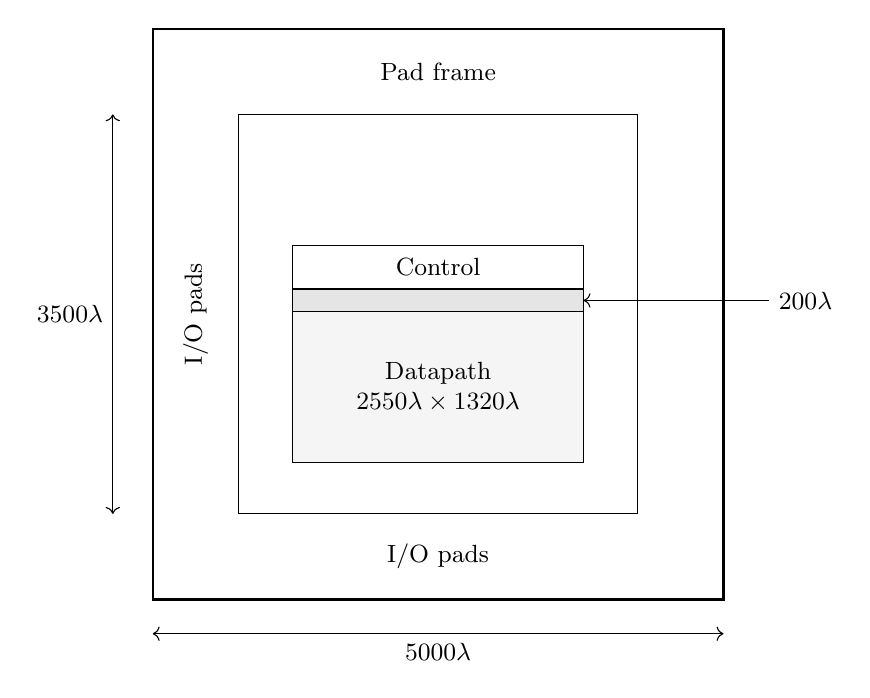
\begin{tikzpicture}[x=0.00145cm,y=0.00145cm,font=\small]
\draw[thick] (0,0) rectangle (5000,5000);
\draw (750,750) rectangle (4250,4250);
\node at (2500,4625) {Pad frame};
\node[rotate=90] at (375,2500) {I/O pads};
\node at (2500,375) {I/O pads};
\draw[fill=gray!8] (1225,1200) rectangle (3775,2520);
\node[align=center] at (2500,1860) {Datapath\\$2550\lambda\times1320\lambda$};
\draw[fill=gray!20] (1225,2520) rectangle (3775,2720);
\draw (1225,2720) rectangle (3775,3100);
\node at (2500,2910) {Control};
\draw[<-] (3775,2620)--(5400,2620) node[right] {$200\lambda$};
\draw[<->] (0,-300)--(5000,-300) node[midway,below] {$5000\lambda$};
\draw[<->] (-350,750)--(-350,4250) node[midway,left] {$3500\lambda$};
\end{tikzpicture}
\end{latin}
\caption{\lr{Floorplan} آموزشی با نسبت ابعاد اصلی کتاب. مستطیل میانی، فضای قابل‌استفاده
داخل \lr{Pad Frame} است. نوار خاکستری کانال کنترل را نشان می‌دهد. جزئیات تک‌تک \lr{Pad}ها حذف شده‌اند
\cite[شکل \secnum{۱.۶۲}]{weste}.}
\label{fig:impl-floorplan}
\end{figure}

\subsection{تبدیل طول و مساحت در مثال کتاب}
در فناوری آموزشی \qty{0.6}{\micro\metre} این مثال، \(\lambda=\qty{0.3}{\micro\metre}\)
است. بنابراین ضلع \(5000\lambda\) برابر \qty{1500}{\micro\metre} یا
\qty{1.5}{\milli\metre} می‌شود. رابطه عمومی تبدیل مساحت چنین است
\begin{equation}
 A_{\mathrm{physical}}=A_{\lambda}\lambda^2.
 \label{eq:impl-area-conversion}
\end{equation}
در این رابطه \(A_{\lambda}\) مقدار عددی مساحت در واحد \(\lambda^2\) است.
چون هر دو بعد طول در \(\lambda\) ضرب می‌شوند، ضریب تبدیل مساحت مربع می‌شود.
در این فناوری، \(1\lambda^2=\qty{0.09}{\micro\metre\squared}\) است.

ابعاد هر \lr{Pad} در کتاب \(750\lambda\times350\lambda\) ذکر شده‌اند.
با کنارگذاشتن حاشیه شعاعی \(750\lambda\) در هر طرف، ضلع فضای داخلی
\(5000-2(750)=3500\lambda\) می‌شود. پس
\begin{align}
 A_{\mathrm{die}}&=(5000\lambda)^2
 =25\times10^6\lambda^2=\qty{2.25}{\milli\metre\squared},\notag\\
 A_{\mathrm{inside}}&=(3500\lambda)^2
 =12.25\times10^6\lambda^2=\qty{1.1025}{\milli\metre\squared}.
 \label{eq:impl-die-core}
\end{align}
مساحت داخل قاب، ظرفیت هندسی موجود را بیان می‌کند. ابعاد بسته پردازنده، شامل دو
بلوک و کانال میان آن‌ها، کوچک‌تر است. با ابعاد گرد‌شده \lr{Floorplan} داریم
\begin{align}
 H_{\mathrm{core}}&=(1320+200+380)\lambda=1900\lambda,\notag\\
 A_{\mathrm{core}}&=(2550)(1900)\lambda^2
 =4.845\times10^6\lambda^2\approx4.8\times10^6\lambda^2.
 \label{eq:impl-core-area}
\end{align}
سهم \lr{Datapath}، کنترل و کانال به‌ترتیب
\(3.366\times10^6\lambda^2\)، \(0.969\times10^6\lambda^2\) و
\(0.510\times10^6\lambda^2\) است. جمع آن‌ها دقیقاً مقدار
\eqref{eq:impl-core-area} را می‌دهد. مقدار فیزیکی متناظر \qty{0.43605}{\milli\metre\squared}
است که برای گزارش تقریبی می‌توان \qty{0.44}{\milli\metre\squared} نوشت.

در این مثال، فضای موردنیاز \lr{Pad Frame} اندازه \lr{Die} را تعیین می‌کند و طراحی
\lr{Pad-limited} است. در طراحی \lr{Core-limited}، اندازه منطق داخلی عامل تعیین‌کننده
مساحت است. کاهش یک بلوک داخلی در حالت اول، تا زمانی که نیاز قاب ثابت بماند،
الزاماً اندازه نهایی \lr{Die} را کاهش نمی‌دهد \cite[صفحه ۴۷]{weste}.

\subsection{گونه‌های ساختار و \lr{Standard Cell}}
کتاب ساختارهای روی تراشه را در گروه‌های \lr{Random Logic}، \lr{Datapath}،
\lr{Array}، \lr{Analog} و \lr{I/O} توضیح می‌دهد \cite[صفحه ۴۸]{weste}.
\lr{Random Logic} اتصال‌های کم‌نظم، مانند \lr{Decoder} منطقی عمومی، دارد.
در \lr{Datapath}، کار مشابه در چند بیت تکرار می‌شود. در \lr{Array}، سلول‌های مشابه
در دو بعد تکرار می‌شوند، مانند \lr{RAM}، \lr{ROM} و \lr{PLA}.
مدار \lr{Analog} و سلول \lr{I/O} به نیازهای الکتریکی و فناوری ویژه خود وابسته‌اند.
تکرار سلولِ طراحی و بررسی‌شده، هزینه طراحی آرایه‌ها را میان نمونه‌های متعدد تقسیم می‌کند.

\lr{Standard Cell} یک سلول کتابخانه‌ای با تابع و هندسه ازپیش‌تعریف‌شده، مانند
\lr{Inverter}، \lr{NAND} یا \lr{Flip-flop}، است. در نمونه کتاب، ریل‌های افقی
تغذیه در \lr{Metal1} عرض \(8\lambda\) و فاصله مرکز تا مرکز \(90\lambda\) دارند.
\lr{nMOS}ها در ناحیه پایین \(40\lambda\) و \lr{pMOS}ها در ناحیه بالای
\(50\lambda\) قرار می‌گیرند. هم‌ترازی ریل و \lr{n-well} امکان اتصال سلول‌های مجاور
از طریق \lr{Abutment} را فراهم می‌کند.

عرض سلول مضربی از \(8\lambda\) است تا تعداد صحیحی مسیر عمودی \lr{Metal2}
داشته باشد. ورودی و خروجی در \lr{Metal2} در دسترس‌اند. \lr{Poly} عمدتاً عمودی و
\lr{Diffusion} و \lr{Metal1} عمدتاً افقی‌اند. اتصال‌های \lr{Substrate} و
\lr{Well} زیر ریل‌ها جا می‌گیرند. فاصله تکرار ردیف‌ها حداقل \(110\lambda\) است.
این اعداد، قواعد کتابخانه آموزشی همان مثال هستند \cite[بخش \secnum{۱.۱۰.۲}]{weste}.

در فرآیند دوفلزی، مسیرهای افقی میان ردیف‌ها به کانال نیاز دارند و تعداد سیم‌ها
ارتفاع کانال را تعیین می‌کند. در مثال سه‌فلزی، \lr{Metal3} افقی با
\lr{Pitch} برابر \(10\lambda\)، روی ارتفاع \(110\lambda\) حدود ۱۱ مسیر فراهم می‌کند.
اگر تقاضای سیم‌کشی در این ظرفیت جا بگیرد، کانال جداگانه می‌تواند حذف شود.
در مثال \lr{MIPS}، جهت‌های غالب \lr{Metal1}، \lr{Metal2} و \lr{Metal3}
به‌ترتیب افقی، عمودی و افقی‌اند. این ترتیب عبور سیم‌ها در لایه‌های مختلف را آسان می‌کند.

کتاب در شکل‌های \secnum{۱.۶۴} و \secnum{۱.۶۵}، نتیجه \lr{Place and Route}
کنترل‌کننده و پردازنده را نشان می‌دهد. نمونه پردازنده در فناوری \qty{130}{\nano\metre}
با هفت لایه فلز، ۲۶ ردیف سلول و حدود \(4\times10^6\lambda^2\) مساحت دارد.
مقایسه تلاش طراحی و سرعت در متن کتاب مربوط به همین زمینه تاریخی است.

\subsection{\lr{Pitch Matching} و \lr{Slice Plan}}
\lr{Pitch} فاصله تکرار یک ساختار است. برای سلول‌هایی که در امتداد یک لبه به هم
می‌چسبند، اندازه و محل اتصال‌های آن لبه باید هماهنگ شوند. این هماهنگی
\lr{Pitch Matching} نام دارد. کوچک‌کردن یک سلول هنگامی که ابعاد نهایی را سلول
همسایه تعیین می‌کند، ممکن است تنها فضای خالی ایجاد کند. بزرگ‌کردن همان سلول نیز
می‌تواند ابعاد همسایه و کل آرایه را افزایش دهد \cite[شکل \secnum{۱.۶۶}]{weste}.

برای نمونه فرضی، چهار سلول با عرض \(w_A\) کنار هم به بلوکی با عرض \(w_B\)
متصل می‌شوند. اگر لبه‌های بیرونی باید هم‌تراز بمانند، عرض موردنیاز ناحیه
\(W=\max(4w_A,w_B)\) است. با \(w_A=20\lambda\) و \(w_B=90\lambda\)،
عرض \(90\lambda\) می‌شود. کاهش \(w_A\) به \(18\lambda\) همچنان همان عرض
نهایی را می‌دهد. برای استفاده از فضای آزاد باید سازمان‌دهی ناحیه نیز بازنگری شود.

\lr{Slice Plan} ترتیب \lr{Wordslice}ها و تخصیص مسیرها در هر \lr{Bitslice} را
پیش از رسم جزئیات مشخص می‌کند. در شکل \secnum{۱.۶۸} کتاب، نقطه روی مسیر بیان می‌کند
که گذرگاه علاوه بر عبور از سلول، در آن سلول مصرف یا تولید می‌شود. پهنای هر جزء با
تعداد مسیر نوشته شده است. بیشترین تراکم این مثال روی \lr{Register File} و برابر
هفت مسیر است \cite[بخش \secnum{۱.۱۰.۴}]{weste}.

جمع عرض اجزای شکل کتاب ۳۱۹ مسیر است. با \lr{Pitch} برابر \(8\lambda\)،
عرض \lr{Datapath} چنین محاسبه می‌شود
\begin{equation}
 W_{\mathrm{data}}=319\times8\lambda=2552\lambda.
 \label{eq:impl-slice-width}
\end{equation}
عدد \(2550\lambda\) در \lr{Floorplan}، مقدار گرد‌شده همین تخمین است.
ارتفاع از هشت \lr{Bitslice}، یک ردیف \lr{Zipper} و سه ردیف \lr{Address Decoder}
ساخته می‌شود. پس با ۱۲ ردیف و فاصله \(110\lambda\)، ارتفاع
\(12(110)\lambda=1320\lambda\) است. فضای خالی ردیف‌های \lr{Decoder} در طراحی
فشرده‌تر می‌تواند برای بخش دیگری مانند کنترل استفاده شود. این تغییر به سازگاری
اتصال و زمان‌بندی نیاز دارد.

\subsection{\lr{Array} و نمونه \lr{PLA}}
\lr{Programmable Logic Array} یا \lr{PLA} توابع به صورت \lr{Sum of Products}
را با دو صفحه پیاده می‌کند. \lr{AND Plane} جمله‌های حاصل‌ضرب و \lr{OR Plane}
ترکیب آن‌ها را می‌سازد. برای نمونه، \(F=ab+ac\) به دو جمله حاصل‌ضرب و یک خروجی
نیاز دارد. در کنترل‌کننده کتاب، این ساختار منطق حالت بعد و خروجی \lr{FSM} را
پیاده می‌کند \cite[بخش \secnum{۱.۱۰.۵}، شکل \secnum{۱.۶۹}]{weste}.

برای قالب آموزشی همان کتاب، هر ورودی دو مسیر عمودی، هر خروجی سه مسیر عمودی و
حاشیه حدود شش مسیر می‌خواهد. هر جمله حاصل‌ضرب حدود یک‌ونیم مسیر افقی و حاشیه
حدود ۱۴ مسیر لازم دارد. اگر \(n_i,n_o,n_p\) به‌ترتیب تعداد ورودی، خروجی و جمله
حاصل‌ضرب و \(p_v,p_h\) فاصله مسیرهای عمودی و افقی باشند، تخمین ساختاری برابر است با
\begin{equation}
 W\approx(2n_i+3n_o+6)p_v,\qquad
 H\approx(1.5n_p+14)p_h.
 \label{eq:impl-pla-estimate}
\end{equation}
فاصله مسیر هر جهت باید از همان قالب سلول تعیین شود. این رابطه رشد عرض با ورودی
و خروجی و رشد ارتفاع با تعداد جمله‌ها را روشن می‌کند.

\lr{PLA} مثال کتاب \(500\lambda\times350\lambda\) است و چهار \lr{Flip-flop}
خارجی ناحیه \(336\lambda\times220\lambda\) دارند. جمع مساحت این دو بخش
\(175000+73920=248920\lambda^2\) می‌شود. مساحت کنترل‌کننده باید سیم‌های ورودی
و خروجی و الزامات جانمایی را نیز در بر بگیرد. برای مقایسه، نمونه کنترل‌کننده حاصل
از ابزار در شکل \secnum{۱.۶۴} ابعاد \(1500\lambda\times400\lambda\) دارد و
بخش بزرگی از آن را کانال‌ها اشغال می‌کنند. این دو سازمان‌دهی و \lr{Floorplan}
بالادستی را با ابعاد و قیود مخصوص خود مقایسه می‌کنیم.

\subsection{تخمین مساحت و دقت اعداد}
تخمین زودهنگام می‌تواند از بلوک مشابه پیشین یا از چگالی تقریبی آغاز شود.
جدول \ref{tab:impl-density} داده‌های جدول \secnum{۱.۱۰} کتاب را با واحد روشن
بازنویسی می‌کند. این اعداد به فناوری، قالب سلول و روش سیم‌کشی وابسته‌اند.
\begin{table}[ht]
\centering
\caption{چگالی‌های تقریبی آموزشی کتاب برای تخمین اولیه \cite[صفحه ۵۲]{weste}.}
\label{tab:impl-density}
\begin{tabularx}{\textwidth}{rX}
\toprule
ساختار & مساحت تقریبی\\
\midrule
\lr{Random Logic} با دو لایه فلز & \(1000\) تا \(1500\lambda^2\) به‌ازای ترانزیستور\\
\lr{Datapath} & \(250\) تا \(750\lambda^2\) به‌ازای ترانزیستور، یا مدل \(6WL+360\lambda^2\)\\
\lr{SRAM} & \(1000\lambda^2\) به‌ازای بیت\\
\lr{DRAM} در فرآیند ویژه آن & \(100\lambda^2\) به‌ازای بیت\\
\lr{ROM} & \(100\lambda^2\) به‌ازای بیت\\
\bottomrule
\end{tabularx}
\end{table}
در مدل \(6WL+360\lambda^2\)، طول‌های \(W,L\) باید با واحد طول سازگار جای‌گذاری
شوند تا \(WL\) مساحت شود. برای حافظه، مساحت بیت‌ها به همراه \lr{Decoder} و مدارهای
جانبی در نظر گرفته می‌شود. تخمین کانال نیز از تعداد مسیر ضرب‌در \lr{Pitch}
آغاز می‌شود. کاهش جزئی سلولی که بارها تکرار می‌شود می‌تواند در سطح کل تراشه اثر
زیادی بگذارد. تخمین محافظه‌کارانه، فضای لازم برای اصلاح و رشد بلوک را فراهم می‌کند.

گاهی چگالی به صورت \lr{kgates/mm²} گزارش می‌شود. کتاب در مثال خود، هر \lr{Gate}
معادل را یک \lr{NAND3} یا \lr{NOR3} شش‌ترانزیستوری می‌گیرد. با این تعریف و
\(\lambda\approx\qty{0.03}{\micro\metre}\)، چگالی
\(160\) تا \(500\) هزار \lr{Gate} در \unit{\milli\metre\squared} به‌ترتیب حدود
\(1160\) تا \(370\lambda^2\) برای هر ترانزیستور می‌دهد
\cite[صفحه ۵۳]{weste}. برای مقدار ۱۶۰ هزار، محاسبه چنین است
\begin{equation}
 a_{\mathrm{tr}}\approx
 \frac{10^6\,\unit{\micro\metre\squared}}
 {160000\times6}\,
 \frac{\lambda^2}{0.03^2\,\unit{\micro\metre\squared}}
 \approx1160\lambda^2.
 \label{eq:impl-density-conversion}
\end{equation}
افزایش چگالی، مساحت متناظر هر ترانزیستور را کاهش می‌دهد. مقایسه دو گزارش چگالی
باید با تعریف یکسان \lr{Gate} و محدوده یکسان سیم‌کشی انجام شود.

\clearpage
\subsection{تمرین‌های پاسخ‌دار \lr{Physical Design}}
\textbf{تمرین ۱.} بلوک فرضی با ۱۰ هزار ترانزیستور و تخمین
\(1000\lambda^2\) برای هر ترانزیستور، در فناوری \(\lambda=\qty{0.1}{\micro\metre}\)
چه مساحتی دارد؟ ابتدا مساحت در واحد \(\lambda^2\) برابر \(10^7\lambda^2\) است.
پس مساحت فیزیکی \(10^7(0.1)^2=10^5\,\unit{\micro\metre\squared}\) یا
\qty{0.1}{\milli\metre\squared} می‌شود. برای فرض مربع‌بودن بلوک، ضلع
\(\sqrt{0.1}\,\unit{\milli\metre}\approx\qty{0.316}{\milli\metre}\) است.
این تخمین باید با محدوده‌ای که چگالی گزارش‌شده پوشش می‌دهد تفسیر شود.

\textbf{تمرین ۲.} برای کانال فرضی ۲۵ مسیر با فاصله \(8\lambda\)، ارتفاع لازم
در مدل کتاب چقدر است؟ حاصل \(25(8)\lambda=200\lambda\) می‌شود.
در \(\lambda=\qty{0.3}{\micro\metre}\)، ارتفاع \qty{60}{\micro\metre} است.
عرض کانال \(2550\lambda\) باشد، مساحت \(510000\lambda^2\) یا
\qty{45900}{\micro\metre\squared} خواهد بود.

\textbf{تمرین ۳.} اگر عرض \lr{Datapath} از ۳۱۹ به ۳۰۰ مسیر برسد و ارتفاع
۱۲ ردیفی ثابت بماند، کاهش مساحت چقدر است؟ عرض جدید \(2400\lambda\) و کاهش
عرض \((319-300)8\lambda=152\lambda\) است. کاهش مساحت برابر
\(152(1320)\lambda^2=200640\lambda^2\)، یعنی حدود ۶ درصد مساحت اولیه
\(2552(1320)\lambda^2\)، می‌شود. تغییر مساحت کل \lr{Die} به عامل تعیین‌کننده
ابعاد نهایی نیز وابسته است.
\clearpage

\section{بررسی درستی طراحی}
\label{sec:book-verification}
\subsection{رابطه میان \lr{Specification} و نمایش‌های طراحی}
\lr{Verification} بررسی می‌کند که طراحی با رفتار و محدودیت‌های مورد انتظار
سازگار باشد. \lr{Specification} باید رفتار خروجی، شرایط ورودی، \lr{Reset}،
زمان‌بندی و سایر قیود لازم را مشخص کند. با دقیق‌ترشدن نمایش، تعداد جزئیات و هزینه
تحلیل افزایش می‌یابد. کتاب برای مدیریت این هزینه، بررسی عملکرد در سطوح بالاتر و
بررسی سازگاری میان نمایش‌های متوالی را توضیح می‌دهد
\cite[بخش \secnum{۱.۱۱}، شکل \secnum{۱.۷۰}]{weste}.

در سطح معماری، مدل رفتاری مانند برنامه \lr{C} با تعریف معماری سنجیده می‌شود.
در سطح منطق، \lr{HDL} با ورودی و خروجی مورد انتظار بررسی می‌شود. در مرحله مدار،
عملکرد شبکه ترانزیستور با تابع منطقی مقایسه می‌شود. در مرحله فیزیکی، اتصال‌های
استخراج‌شده از \lr{Layout} با \lr{Schematic} مقایسه می‌شوند. در کنار این زنجیره،
مدار و \lr{Layout} باید قیود زمان‌بندی و توان را برآورده کنند.

برای نمونه، اگر نیاز سیستم جمع هشت‌بیتی با \lr{Carry-out} باشد، رفتار مرجع باید
جمع کامل ۹ بیتی را مشخص کند. سپس خروجی هشت‌بیتی، هشت بیت کم‌ارزش نتیجه و
\lr{Carry-out} بیت نهم است. اگر تعریف علامت‌دار بودن داده یا رفتار \lr{Overflow}
مبهم بماند، پاسخ مورد انتظار آزمون نیز مبهم می‌شود.

\subsection{\lr{Testbench} و انتخاب ورودی‌ها}
\lr{Testbench} محیطی است که \lr{Device Under Test} یا \lr{DUT} را نمونه‌سازی
می‌کند، ورودی‌ها را اعمال می‌کند و پاسخ را با مرجع مقایسه می‌کند. یک \lr{Test Vector}
می‌تواند شامل ورودی و پاسخ مورد انتظار باشد. در مدار ترتیبی، زمان اعمال ورودی،
\lr{Clock}، \lr{Reset} و وضعیت قبلی نیز بخشی از سناریو هستند
\cite[صفحه ۵۳]{weste}.

برای تابع ترکیبی با \(n\) ورودی دودویی، تعداد حالت‌ها \(2^n\) است، زیرا برای هر
ورودی دو انتخاب مستقل داریم. \lr{Carry} سه‌ورودی ۸ حالت دارد. جمع‌کننده هشت‌بیتی
با دو عملوند هشت‌بیتی و یک \lr{Carry-in}، تعداد
\(2^{8+8+1}=131072\) حالت دارد. با افزایش ورودی‌ها، بررسی کامل به‌سرعت پرهزینه
می‌شود. برای مدار ترتیبی، ترتیب ورودی‌ها و حالت داخلی نیز باید بررسی شوند.

در نمونه آموزشی، برای جمع‌کننده ورودی‌های صفر، بیشینه مقدار، تولید و انتشار
\lr{Carry} و الگوهای مکمل ارزش بررسی دارند. در پردازنده، \lr{Reset}، هر نوع دستور،
شاخه گرفته‌شده و گرفته‌نشده و مرز نشانی‌ها باید طبق تعریف معماری آزموده شوند.
پاسخ مرجع باید از صورت مسئله و محاسبه مستقل به دست آید. کپی همان عبارت اشتباه
از طراحی به مرجع می‌تواند همان خطا را در هر دو حفظ کند.

\lr{Post-synthesis Netlist} را می‌توان با بردارهای آزمون قبلی شبیه‌سازی کرد.
برای شبکه ترانزیستور نیز آزمون عملکرد ممکن است. در مدار ترتیبی، ترتیب رخدادها و
\lr{Race Condition} اهمیت پیدا می‌کند. ابزار \lr{Formal Verification} نیز می‌تواند
تحت فرض‌ها و مدل تعریف‌شده، هم‌ارزی تابع یا خاصیت را بررسی کند.
کیفیت فرض‌ها و پوشش حالت‌ها بر معنای نتیجه اثر می‌گذارد.

\subsection{\lr{DRC}، \lr{LVS}، \lr{ERC} و تحلیل الکتریکی}
\lr{Design Rule Check} یا \lr{DRC} هندسه را با قواعد فناوری مقایسه می‌کند، مانند
حداقل عرض، فاصله و پوشش اتصال. \lr{Layout Versus Schematic} یا \lr{LVS} بررسی
می‌کند که ترانزیستورها و اتصال‌های استخراج‌شده از \lr{Layout} با مدار مرجع سازگار
باشند. \lr{Electrical Rule Check} یا \lr{ERC} برای یافتن مسئله‌های الکتریکی
تعریف‌شده در مجموعه قواعد به کار می‌رود. کتاب به مشکلاتی مانند نویز یا فرسودگی
زودهنگام اشاره می‌کند \cite[صفحه ۵۳]{weste}.

جدول \ref{tab:impl-verification} مثال‌هایی از ارتباط خطا و بررسی مناسب را نشان می‌دهد.
یک مسئله ممکن است در بیش از یک بررسی آشکار شود و توان کشف هر ابزار به مدل و قواعدش وابسته است.
\begin{table}[ht]
\centering
\caption{نمونه ارتباط مسئله طراحی با بررسی لازم.}
\label{tab:impl-verification}
\begin{tabularx}{\textwidth}{rX}
\toprule
مسئله & بررسی مرتبط\\
\midrule
اشتباه در تابع \lr{Carry} & مقایسه رفتاری، جدول کامل یا بررسی هم‌ارزی\\
سیم با عرض کمتر از حد مجاز & \lr{DRC} با قواعد فناوری\\
اتصال خروجی به گره داخلی اشتباه & \lr{LVS} در برابر مدار مرجع\\
اتصال الکتریکی نامناسب تغذیه یا \lr{Body} & \lr{ERC} و بررسی اتصال با قواعد مرتبط\\
رسیدن خروجی پس از مهلت لازم & تحلیل زمان‌بندی با مدل مناسب مدار و سیم\\
مصرف توان بیشتر از بودجه & تحلیل توان با تحریک، فعالیت و مدل معتبر\\
\bottomrule
\end{tabularx}
\end{table}

اگر هندسه قانونی باشد اما دو گره منطقی جابه‌جا شده باشند، ممکن است
\lr{DRC} بدون خطای هندسی پایان یابد و \lr{LVS} اختلاف اتصال را پیدا کند.
اگر اتصال با مرجع برابر باشد اما خود مرجع تابع اشتباه داشته باشد، مقایسه رفتاری
با \lr{Specification} لازم است. برای بررسی سرعت و توان نیز مقاومت و خازن سیم،
اندازه ترانزیستور، ولتاژ و شرایط مدل‌شده اهمیت دارند.

\subsection{تمرین‌های پاسخ‌دار \lr{Verification}}
\textbf{تمرین ۱.} در گیت \lr{NAND2}، خروجی در \lr{Layout} به \(V_{DD}\) اتصال
پیدا کرده است. آزمون عملکرد چه ورودی‌ای را باید حتماً اعمال کند؟
برای \(a=b=1\)، پاسخ مرجع صفر است. خروجی ثابت یک اختلاف را آشکار می‌کند.
سه حالت دیگر خروجی مرجع یک دارند و این خطا را در مدل خروجی ثابت نشان نمی‌دهند.
\lr{LVS} نیز باید اختلاف اتصال با مدار صحیح را بررسی کند.

\textbf{تمرین ۲.} مدار تابع درست را با تأخیر \qty{2}{\nano\second} تولید می‌کند،
ولی مهلت داده‌شده \qty{1.5}{\nano\second} است. نتیجه چیست؟
شرط عملکرد منطقی برآورده شده، اما قید زمان‌بندی \qty{0.5}{\nano\second} نقض شده است.
برای اعلام موفقیت باید هر دو شرط تابع و مهلت برقرار باشند.

\textbf{تمرین ۳.} آیا یک آزمون موفق برنامه \lr{Fibonacci}، همه حالت‌های پردازنده
را پوشش می‌دهد؟ این برنامه تنها توالی مشخصی از دستورها، داده‌ها و شاخه‌ها را طی
می‌کند. برای پوشش نیازهای دیگر باید سناریوهای متناسب با همان نیازها افزوده شود.
مثلاً صحت \lr{Reset}، دستور استفاده‌نشده و حالت مرزی \lr{Branch} به بررسی مربوط خود نیاز دارد.
\clearpage

\section{ساخت، \lr{Packaging} و \lr{Testing}}
\label{sec:book-manufacturing}
\subsection{\lr{Tapeout}، \lr{Mask} و تقسیم هزینه ساخت}
پس از نهایی‌شدن طراحی و بررسی‌های لازم، توصیف هندسه ماسک‌ها برای ساخت تحویل
داده می‌شود. این مرحله \lr{Tapeout} نام دارد. نام آن از روش تاریخی تحویل داده روی
نوار مغناطیسی آمده است. کتاب قالب‌های \lr{Caltech Interchange Format} یا
\lr{CIF} و \lr{Calma GDS II Stream Format} یا \lr{GDS} را معرفی می‌کند
\cite[بخش \secnum{۱.۱۲}]{weste}.

\lr{Mask} الگوی لازم برای انتقال هندسه یک مرحله از فرآیند را فراهم می‌کند.
کتاب روش ساخت الگوی کروم روی شیشه با پرتو الکترونی را توضیح می‌دهد.
هزینه ماسک و تجهیز خط تولید، بخش مهمی از هزینه ثابت ساخت است.
متن سال ۲۰۱۱ برای مثال‌های \qty{180}{\nano\metre} و \qty{65}{\nano\metre}
به‌ترتیب حدود ۲۵۰ هزار و ۳ میلیون دلار هزینه مجموعه ماسک ذکر می‌کند.
این مقادیر، مثال تاریخی همان کتاب‌اند.

در \lr{Multi-project Wafer}، چند طراحی کوچک از مجموعه مشترکی از ماسک‌ها استفاده
می‌کنند تا هزینه ثابت میان مشتریان تقسیم شود. کتاب خدمات \lr{MOSIS}،
\lr{EUROPRACTICE} و \lr{VDEC} را در زمینه زمان انتشار معرفی می‌کند.
در مدل آموزشی فرضی، اگر هزینه ثابت مشترک \(K\) میان \(N\) طراحی با سهم برابر
تقسیم شود، سهم هر طراحی \(K/N\) است. هزینه عملی به سهم سطح، فرآیند، تعداد نمونه،
\lr{Packaging} و شرایط خدمات وابسته است.

\lr{Fab} کارخانه ساخت و \lr{Foundry} تأمین‌کننده خدمات ساخت است.
شرکت \lr{Fabless} طراحی را انجام می‌دهد و ساخت را به کارخانه طرف قرارداد می‌سپارد.
کتاب هزینه بالای تأسیس کارخانه و اهمیت اقتصادی این تقسیم کار را توضیح می‌دهد.

\subsection{از \lr{Wafer} تا \lr{Die}}
روی یک \lr{Wafer} سیلیکونی، تعداد زیادی نسخه مدار هم‌زمان ساخته می‌شوند.
مراحل تکراری رسوب‌دهی، ماسک‌گذاری، \lr{Etch} و \lr{Implant} همان هندسه و
ساختار افزاره را ایجاد می‌کنند که در بخش ساخت مقدماتی آموختیم.
کتاب قطرهای \qty{150}{\milli\metre} تا \qty{300}{\milli\metre} و زمان بازگشت
تا حدود ۱۰ هفته را برای زمینه صنعتی زمان خود شرح می‌دهد \cite[صفحه ۵۴]{weste}.

در \lr{Clean Room}، فیلتر هوا و پوشش کارکنان، ورود ذرات آلاینده را کاهش می‌دهد.
یک ذره کوچک می‌تواند بخشی از الگو را خراب کند و اتصال باز یا اتصال کوتاه بسازد.
پس از فرآوری، \lr{Wafer} به قطعه‌های \lr{Die} بریده می‌شود. هندسه نهایی قطعه،
تعداد و محل اتصال‌ها و نیاز حرارتی، در انتخاب \lr{Package} نقش دارند.

\subsection{\lr{Wire Bonding} و \lr{Flip-chip}}
\lr{Package} اتصال قابل‌استفاده با محیط بیرونی و حفاظت مکانیکی قطعه را فراهم
می‌کند و در دفع گرما و رفتار الکتریکی نیز نقش دارد. مثال \lr{MIPS} کتاب، قطعه
\qty{1.5}{\milli\metre} در \qty{1.5}{\milli\metre} را در \lr{Dual-inline Package}
یا \lr{DIP} با ۴۰ پایه نشان می‌دهد. در \lr{Wire Bonding}، سیم‌های نازک طلا
\lr{Pad}های قطعه را به \lr{Lead Frame} بسته وصل می‌کنند
\cite[شکل \secnum{۱.۷۳} و صفحه ۵۵]{weste}.

در \lr{Flip-chip}، اتصال‌های لحیمی کوچک روی سطح قطعه ایجاد می‌شوند و قطعه
روبه‌پایین به زیرلایه متصل می‌شود. امکان توزیع اتصال‌ها در سطح تراشه، ظرفیت اتصال
را افزایش می‌دهد. حذف سیم \lr{Bond Wire} سهم القایی آن سیم را از مسیر برمی‌دارد.
رفتار الکتریکی نهایی همچنان به کل مسیر اتصال و بسته وابسته است.
کتاب معیارهای هزینه، تعداد پایه، پهنای باند پایه، انتقال توان و قابلیت اطمینان را
برای مقایسه بسته‌ها مطرح می‌کند و جزئیات را به فصل ۱۳ ارجاع می‌دهد.

\subsection{آزمون قطعه ساخته‌شده و \lr{BIST}}
\lr{Testing} قطعه ساخته‌شده را با معیار پذیرش می‌سنجد تا نمونه‌های دارای عیب
شناسایی شوند. حتی با طراحی صحیح، نقص ساخت یا آلودگی می‌تواند قطعه معیوب ایجاد کند.
آزمون به دسترسی ورودی‌ها، مشاهده پاسخ‌ها، سرعت موردنظر و هزینه زمانی دستگاه
آزمون وابسته است \cite[صفحه ۵۵]{weste}.

در \lr{Built-in Self-test} یا \lr{BIST}، مدارهای کمکی روی تراشه بخشی از تولید
تحریک و بررسی پاسخ را انجام می‌دهند. هدف معرفی‌شده در کتاب کاهش زمان لازم
دستگاه آزمون خارجی است. این انتخاب، منطق و مساحت کمکی می‌خواهد.
پوشش عیب به روش تولید الگو و تحلیل پاسخ وابسته است.
معیار آزمون باید با عیب‌هایی که قصد کشفشان را داریم متناسب باشد.

برای تحلیل اقتصادی ساده، \lr{Yield} را نسبت تعداد قطعات سالم به تعداد قطعات
ساخته‌شده تعریف می‌کنیم. اگر به فرض ۱۰۰۰ قطعه ساخته شود و ۸۵۰ قطعه معیار پذیرش
را برآورده کنند، \(Y=850/1000=0.85\)، یعنی ۸۵ درصد است.
اگر هزینه مفروض همین مرحله \(K\) باشد، هزینه سرشکن‌شده هر قطعه سالم در این مدل
\begin{equation}
 C_{\mathrm{good}}=\frac{K}{N_{\mathrm{good}}}
 =\frac{K}{YN_{\mathrm{total}}}
 \label{eq:impl-yield-cost}
\end{equation}
خواهد بود. \(N_{\mathrm{total}}\) تعداد کل و \(N_{\mathrm{good}}\) تعداد سالم است.
با ثابت‌بودن هزینه و تعداد ساخت، کاهش \lr{Yield} هزینه هر قطعه سالم را افزایش می‌دهد.
این مثال افزوده، مدل سرشکن‌کردن یک هزینه مشخص است. هزینه‌های مراحل دیگر باید
در مدل اقتصادی کامل خود لحاظ شوند.

\subsection{تمرین‌های پاسخ‌دار ساخت و آزمون}
\textbf{تمرین ۱.} هزینه فرضی یک مرحله برای ۱۰۰۰ قطعه، ۲۰ هزار واحد پول است.
با \lr{Yield} برابر ۸۰ درصد، هزینه همان مرحله برای هر قطعه سالم چقدر می‌شود؟
تعداد سالم \(0.8(1000)=800\) و هزینه واحد \(20000/800=25\) واحد پول است.
با \lr{Yield} برابر ۵۰ درصد، هزینه \(20000/500=40\) واحد پول می‌شود.

\textbf{تمرین ۲.} برای عیب خروجی گیرکرده روی صفر در \lr{Carry}، چه ورودی‌ای مناسب است؟
مثلاً \(a=b=1,c=0\) پاسخ مرجع یک دارد و عیب را در مدل گیرکردن خروجی آشکار می‌کند.
ورودی \(0,0,0\) پاسخ مرجع صفر دارد و این عیب خاص را آشکار نمی‌کند.
همان منطق انتخاب تحریک در \lr{Testbench} نیز کاربرد دارد.

\textbf{تمرین ۳.} اگر \lr{LVS} و آزمون عملکرد پیش از ساخت موفق باشند، قطعه ساخته‌شده
چه بررسی دیگری می‌خواهد؟ شرایط ساخت هر نمونه می‌تواند نقص ایجاد کند، بنابراین
آزمون قطعه با معیارهای عملکرد و کیفیت تعیین‌شده لازم است. صحت اتصال استخراج‌شده،
صحت رفتار مدل و سلامت نمونه فیزیکی، هر یک به شواهد مناسب خود وابسته‌اند.

\subsection{پیوند این بخش با مدل‌های فصل ۲}
برای محاسبه دقیق‌تر تأخیر باید بدانیم جریان ترانزیستور چگونه به
\(V_{GS}\)، \(V_{DS}\)، \(V_{BS}\)، \(W\) و \(L\) وابسته است.
برای محاسبه بار باید خازن‌های \lr{Gate}، \lr{Diffusion} و سیم را بشناسیم.
برای ارزیابی حالت منطقی پایدار نیز رابطه ورودی و خروجی \lr{Inverter} اهمیت دارد.
بخش‌های آغازین فصل ۲ این مدل‌های افزاره را می‌سازند و بخش‌های بعدی اثرهای غیرایده‌آل
و مشخصه‌های \lr{DC} را به آن‌ها اضافه می‌کنند.
\clearpage

\begin{thebibliography}{9}
\bibitem{weste}
\begin{latin}
Neil H. E. Weste and David Money Harris,
\textit{CMOS VLSI Design: A Circuits and Systems Perspective},
Fourth Edition, Pearson, 2011.
\end{latin}
بخش \secnum{۱.۹} در صفحات چاپی ۴۲ تا ۴۵، بخش \secnum{۱.۱۰} در صفحات ۴۵ تا ۵۳،
بخش \secnum{۱.۱۱} در صفحه ۵۳ و بخش \secnum{۱.۱۲} در صفحات ۵۴ و ۵۵ بررسی شده‌اند.
شماره صفحه فایل \lr{PDF} برابر شماره چاپی به‌اضافه ۲۷ است.
شکل‌های \secnum{۱.۶۰} تا \secnum{۱.۷۳} و جدول \secnum{۱.۱۰} مبنای تطبیق‌اند.
شکل‌های جزوه بازترسیم آموزشی با شماره مستقل هستند.
\bibitem{intro}
اسلایدهای محلی \lr{Introduction}، فایل \lr{00-introduction.pdf}، اسلاید ۱۷ درباره سطوح طراحی.
اصل یادداشت‌ها طبق اسلاید ۲ متعلق به \lr{David Money Harris}، سال ۲۰۱۱، و نسخه محلی اقتباس‌شده است.
\end{thebibliography}
\end{document}
